\documentclass[12pt]{article}
\usepackage[utf8]{inputenc}
\usepackage[russian]{babel}
\usepackage{graphicx}
\usepackage{listings}
\usepackage{indentfirst}

\newcommand{\rot}{\mathop{\rm rot}\nolimits}
\

\title{Сравнение наборов конечных элементов для стационарной задачи о каверне с подвижной верхней границей}
\date{Ноябрь 2012}
\author{Виктор Борисов}

\begin{document}

\maketitle

\section{Задача}
В данном разделе представлены стационарные уравнения Стокса, 
постановка задача и течении в каверне и рассматриваемы конечные элементы.
\subsection{Стационарные уравнения Стокса}
Стационарные уравнения Стокса описывают устоявшееся несжимаемое течение в области $\Omega$ с границей $\delta\Omega$
\begin{equation}
-\Delta u + \nabla p = f \quad x \in \Omega,
\end{equation}
\begin{equation}
\nabla\cdot u = 0 \quad x \in \Omega,
\end{equation}
\begin{equation}
u = g \quad x \in \partial\Omega,
\end{equation}
где $u$ - поле скоростей, $p$ - поле давления и $f$ - внутренний источник движения.
В этой постановке присутствуют две зависимые неизвестные: скорость и давление.
В численном решении этого и вообще всех уравнений типа Навье-Стокса, используемые конечные элементы должны удовлетворять условию Ладыженской-Бабушки-Бреззи. Часто используемые полиномы Лагранжа второго порядка для давления и скорости приводят к несходимости решения.

\subsection{Задача о течении в каверне}
В качестве тестовой задачи рассматривается двумерная задача о течении в каверне с подвижной верхней границей. Верхняя граница конечно неподвижна, но поле скоростей на ней имеет определенное значение. Постановка и решение тестовой задачи не имеют физических единиц измерения. Мы рассматриваем единичный квадрат $\Omega$ (рис. \ref{fg:cavity}), где на верхней границе $\partial\Omega_{top}$ поле скоростей принимает значения $u_x=1$ и $u_y=0$, в остальной части границы $\partial\Omega_{wall}$ поле скоростей $u=0$ (условие неприлипания).
С добавлением таких граничных условий, уравнения принимают следующий вид:
\begin{equation}
-\Delta u + \nabla p = f \quad x \in \Omega,
\end{equation}
\begin{equation}
\nabla\cdot u = 0 \quad x \in \Omega,
\end{equation}
\begin{equation}
u = (1, 0) \quad x \in \partial\Omega_{top},
\end{equation}
\begin{equation}
u = (0, 0) \quad x \in \partial\Omega_{wall}.
\end{equation}

\begin{figure}
	\begin{center}
		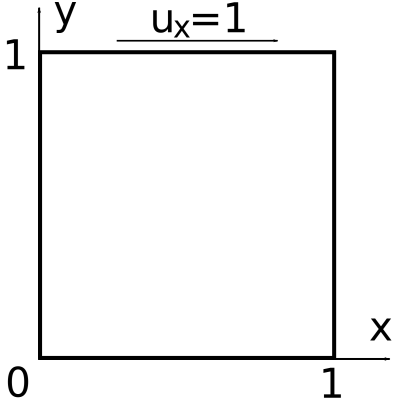
\includegraphics[width=200px]{pics/cavity400}
		\caption{Тестовая область с подвижной верхней границей.}
		\label{fg:cavity}
	\end{center}
\end{figure}

\subsection{Конечные элементы}
Для численного решения методом конечных элементов, для начала систему уравнений переписывают в вариационную постановку:
\begin{equation}
a(u,v)-b(v,p)=(f,v) \quad \forall v \in V,
\end{equation}
\begin{equation}
b(u,q)=0 \quad \forall q \in \Pi,
\end{equation}
где 
\begin{equation}
a(u,v)=\int_\Omega \nabla v \cdot \nabla v \, dx,
\end{equation}
\begin{equation}
b(v,q)=\int_\Omega (\nabla \cdot v) q \, dx,
\end{equation}
\begin{equation}
(f,v)=\int_\Omega f \cdot v \, dx.
\end{equation}
В этой постановке множества $V$ и $\Pi$ это функциональные пространства для скорости и давления соответственно. Эти пространства состоят из конечных элементов, выбор которых влияет на качества решения. Рассматриваются три набора элементов: Taylor Hood (TH), continious discontinious Lagrange (CD), Crouzeix Raviart (CR). 

Набор TH состоит из двух полиномов Лагранжа (Lagrange) для скорости и давления. Причем порядок полинома для скорости на единицы выше чем для давления. На рис. \ref{fg:lagrange2} элемент второго порядка, для первого порядка исчезают точки по середине сторон треугольника.

Набор CD состоит из полином Лагранжа порядка 2 для скорости и разрывного полинома Лагранжа (Discontinuous Lagrange) порядка 0.

Набор CR это элемент Crouzeix Raviart для скорости и разрывный полином Лагранжа порядка 0 для давления. На рис. \ref{fg:crouzeix1} представлен элемент первого порядка. Точки определяющие степени свободы расположены не на концах треугольника, а на середине сторон.

Набор TH и CD имеют максимум второй порядок, а CR первый (табл. \ref{tb:order}), что будет сказываться на свойствах решения.

\begin{figure}
	\begin{center}
		\includegraphics[width=200px]{pics/lagrange2}
		\caption{Элемент Лагранжа второго порядка.}
		\label{fg:lagrange2}
	\end{center}
\end{figure}

\begin{figure}
	\begin{center}
		\includegraphics[width=200px]{pics/crouzeix1}
		\caption{Элемент Crouzeix Raviart первого порядка.}
		\label{fg:crouzeix1}
	\end{center}
\end{figure}

\begin{table}
\begin{center}
\begin{tabular}{|c|c|c|}
\hline
Название & Скорость & Давление \\
\hline
TH & 2 & 1 \\
\hline
CD & 2 & 0 \\
\hline
CR & 1 & 0 \\
\hline
\end{tabular}
\end{center}
\caption{Порядки элементов для скорости и давления}
\label{tb:order}
\end{table}

\section{Решение}
В данном разделе описывается используемый способ сравнения решений полученных с помощью различных наборов конечных элементов. Используется функция тока, как показатель решения двумерной задачи с вычислением поля скоростей. Приводится отрывок из программы на языке Python с использованием библиотеки Fenics.

\subsection{<<Точное>> решение}
Не обладая точным решением в задаче о каверне, мы должны с чем-то сравнивать полученные результаты. Поэтому <<точным>> решением будем считать результат полученный на мелкой сетке. Все выбранные наборы элементов должны сходиться к этому <<точному>> решению при выборе мелкой сетки. Исходная область (единичный квадрат) делиться на $h^2$ квадратов, и каждый квадрат делится на два треугольника. Этот $h$ будем считать размером сетки.

За <<точное>> решение возьмем результат полученный набором TH на сетке размером $h=200$. В дальнейшем <<точное>> решение употребляется без кавычек.

\subsection{Функция тока}
В задачах с вычислением поля скоростей одним из общепринятых показателей является функция тока. Визуальное сравнение поля скоростей для двумерной задачи не очевидное, потому вместо двумерных векторов скорости - сравнивают одномерную функцию тока. Функция тока обладает следующими свойствами:
\begin{equation}
u_x = \frac{\partial \psi}{\partial y},
\end{equation}
\begin{equation}
u_y = - \frac{\partial \psi}{\partial x}.
\end{equation}
Чтобы вычислить $\psi$, надо решить уравнение Лапласа:
\begin{equation}
\Delta\psi=-\xi,
\end{equation}
где $\xi=\rot U$ - вектор вихря.

\subsection{Сравниваемые свойства наборов элементов}
Вычисляются решения на разных сетках, изменяя параметр $h$ и наборы конечных элементов указанных выше.
Нас интересует во-первых время и точность вычисления решения.

Время вычисления $t$ это количество времени потраченное на решение общей системы линейных уравнений.

Точность вычисления это разница между точным и текущим решениями, что такое точное решение указано выше. Разницу для скорости $u_{err}$, давления $p_{err}$, функции тока $\psi_{err}$ мы берем следующим образом:
\begin{equation}
u_{err} = \int_{\Omega} (u_{ex} - u, u_{ex} - u) dx,
\end{equation}
\begin{equation}
p_{err} = \int_{\Omega} (p_{ex} - p, p_{ex} - p) dx,
\end{equation}
\begin{equation}
\psi_{err} = \int_{\Omega} (\psi_{ex} - \psi, \psi_{ex} - \psi) dx,
\end{equation}
где $u_{ex}$, $p_{ex}$, $\psi_{ex}$ соответствующие точные решения.

\subsection{Программа}
Программа составлена на языке Python с помощью библиотеки Fenics.
\begin{lstlisting}
elements_table = {
    "CR": ("Crouzeix-Raviart", 1, "Discontinuous Lagrange", 0),    
    "CD": ("Lagrange", 2, "Discontinuous Lagrange", 0),    
    "TH": ("Lagrange", 2, "Lagrange", 1),
}
\end{lstlisting}

\section{Результаты}
\subsection{Графики}
\subsection{Выводы}


\end{document}